% 15 de mayo de 2018
\chapter{Presentación y discusión de la información}\label{ch:informacion}

El proceso de entrevistas fue realizado entre los meses de abril y septiembre
del año 2017.
Estas entrevistas fueron transcritas para su análisis en el texto.
Los elementos expresados por los participantes en las entrevistas fueron
codificados y organizados en las categorías y subcategorías que se pueden
observar en la figura~\ref{fig:categorias}.
Las entrevistas fueron codificadas empleando el programa ATLAS.ti en su versión
7.5.7 proceso que facilitó la categorización de la información recolectada a lo
largo de las entrevistas.

\begin{figure}
    \centering
    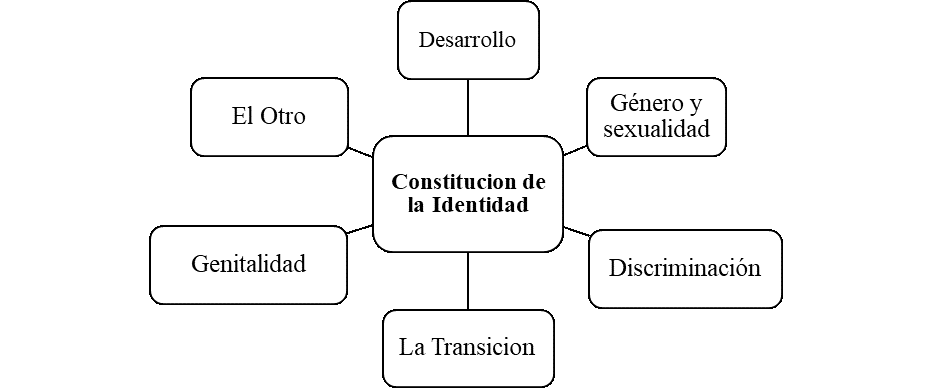
\includegraphics[width=0.75\textwidth]{categorias}
    \caption{Diagrama de categorías}\label{fig:categorias}
\end{figure}

A continuación realizaremos una descripción de cada una de ellas junto con los
verbatim que les dan origen.
Adicionalmente presentamos el razonamiento e interpretación que damos a cada
categoría y sus implicaciones caso a caso para el cumplimiento de los objetivos
de investigación.
El orden de presentación de las mismas fue elegido
según la frecuencia de manifestación en las entrevistas realizadas.

En la sección~\ref{sec:discusion}, realizamos una discusión y análisis punto a
punto de cada una de las categorías.

\section{Presentación de la información}

Como se puede ver resumido en la figura~\ref{fig:categorias}, hemos elaborado
seis (6) categorías. Dentro de estas categorías ‘La transición’ es uno de los
componentes identificados como constitutivo del proceso de construcción de la
identidad de las personas trans. Procederemos a explorar el contenido de cada
una de las categorías identificadas.

\subsection{Desarrollo}
Esta categoría se encuentra compuesta por elementos que abarcan desde etapas
tempranas de la niñez y del desarrollo.
Elementos como la relación del individuo con su escolaridad y compañeros de
clases.
También elementos de la constitución de los géneros que se hacen presentes
dentro de la pubertad y los conflictos que estos puedan causar a los
participantes
También incluye el papel que juega la familia dentro de la constitución de la
identidad así como la forma de aproximarse a los problemas.
Todos estos son elementos que pueden marcar la construcción de identidad de una
persona.

\begin{figure}
    \centering
    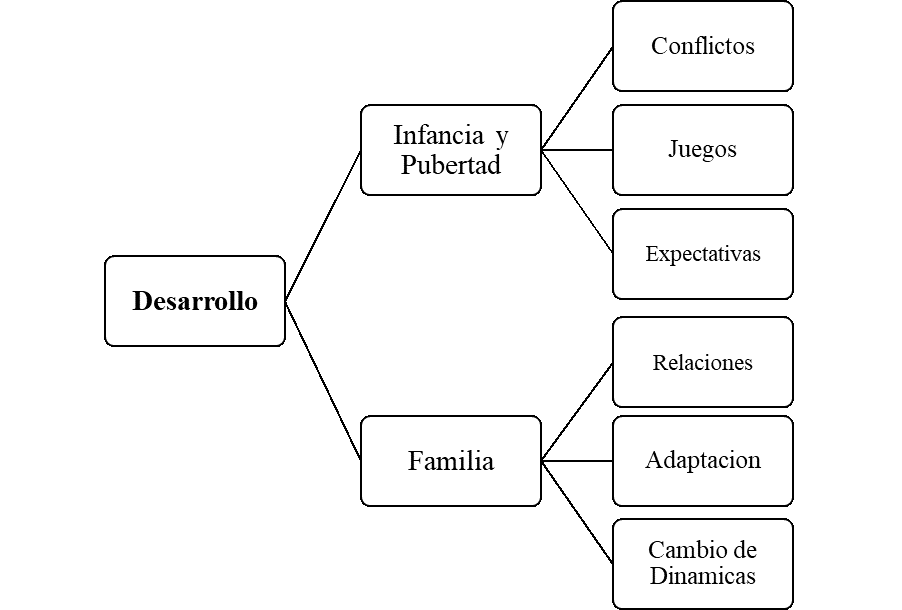
\includegraphics[width=0.75\textwidth]{desarrollo}
    \caption{Diagrama ‘desarrollo y familia’}\label{fig:desarrollo}
\end{figure}

En esta categoría confluyen elementos de conflicto así como las experiencias que
permitieron el manejo de los mismos en los participantes y que
consecuentemente se transformaron en estrategias de afrontamiento. Se debe tomar
en cuenta que en esta categoría se presentan los distintos tipos de relación
establecidas tanto en niveles académicos como familiares entre la infancia y
pubertad de los participantes.

Existen dos subcategorías dentro de este factor. Una de ‘infancia y pubertad’,
que reporta sobre las experiencias de desarrollo y formativas en la juventud, y
otra de ‘familia’. Esta habla acerca de la influencia de los lazos y ambiente
familiar durante el desarrollo.

\subsubsection{Infancia y pubertad}
Dentro de esta subcategoría se pueden
encontrar elementos que parecen ser transversales a lo largo de la vida del
individuo. Al ser tanto la infancia como la pubertad etapas tempranas de
desarrollo y constitución se pudo identificar elementos que parecen sentar las
bases para la forma otros elementos que le permiten al individuo constituirse
como persona. Entre estos elementos cabe resaltar la presencia de conflictos
como lo expresa el caso~1 (verbatim):

\begin{verbatim}
…bueno me identificaba como niño pero me gustaba todo las cosas
de niña. De hecho siempre pedía al niño Jesús cosas de hembra, por ejemplo,
barbie, oso etcétera. Por su puesto, jamás me traía lo que pedía y era muy
triste para mí, una era inocente y el niño Jesús me dejaba una carta explicando
que eso eran cosas de niña y me traía patineta bicicleta carrito y a mí no me
gustaba…
\end{verbatim}

Este elemento puede estar ligado al rechazo que pueden vivir, según lo expresado
por el caso~1 (verbatim):

\begin{verbatim}
…en la escuela era algo terrible por el bullying, pero yo
siempre imponía carácter y jamás me deje amedrentar por nada ni nadie. De hecho
me agarre a golpes y me expulsaron por 10 días…
\end{verbatim}

O a tener su raíz en conflictos por la constitución de su identidad como lo
expresan con los siguientes verbatims.

Caso~1:

\begin{verbatim}
…yo lloraba porque no me entendía y me sentía mal.
\end{verbatim}

Caso~2:

\begin{verbatim}
  …me criticaban mucho como me vestía, pero es lo que me gusta.
\end{verbatim}

Y caso~3:

\begin{verbatim}
…siempre era el raro del grupo…
\end{verbatim}

La aparición de estos conflictos entra en contacto con las aproximaciones a los
roles de género que suceden por primera vez en la infancia por medio de los
juegos y que perduran a lo largo de la vida de un individuo, como se evidencia
en el relato del caso~1:

\begin{verbatim}
…a mí me decían que tenía que jugar con carritos y no con
muñecas porque eso es de niñas y yo no era una…
\end{verbatim}

Y del caso~3:

\begin{verbatim}
…me gustaba tener el cabello corto y no me arreglaba pero mis
padres me decían que tenía que arreglarme para poder verme linda…
\end{verbatim}

 Un elemento que se ve relacionado con la presencia del conflicto de identidad
 es que la aprehensión del mismo lleva al individuo a buscar o considerar el
 daño que puede causar el no lidiar con esta situación y es por eso que hay
 comentarios como el emitido por el caso~3 quien expresa sobre su
 adolescencia:

 \begin{verbatim}
Descubrí que tenía que hablar de esto con alguien o me iba a volver loco.
 \end{verbatim}

 Este verbatim, trae a la luz el malestar que nace en el individuo por este
 conflicto de identidad, posiblemente el hecho de estar en una situación de la
 cual se tiene poca o ninguna información al alcance del individuo hace que el
 malestar por el conflicto sea mayor y pueda tener consecuencias mas peligrosas
 para la identidad de la vida del individuo.

\subsubsection{Familia}

Otro de los componentes de la categoría ‘Desarrollo’ es la subcategoría
denominada \emph{Familia}, pues según lo expresado por los participantes como
caso~3:

\begin{verbatim}
…en mi casa siempre era un conflicto hablar sobre cómo me sentía.
\end{verbatim}

Caso~2:

\begin{verbatim}
Mi mamá me decía, ‘hija arréglate un poco’ ó ‘te verías muy linda
con vestido’ y yo le decía que no me gustaba eso y venía el regaño.
\end{verbatim}

Esta subcategoría influye en la constitución del individuo y modela su
desarrollo, en aspectos como la forma de establecer relaciones,
tomando lo expresado por el caso~2:

\begin{verbatim}
…la relación con mis padres es distinta, a mi madre le costó más
aceptarme. A mi padre, después de explicarle, lo entendió con más facilidad,
incluso suelo pasar por su trabajo, es moto taxista.
\end{verbatim}

Un elemento que resaltan los participantes es el cambio de dinámicas dentro de
la familia que se da producto de asumirse como persona trans. Como se observa en
el relato de caso~1:

\begin{verbatim}
…mi madre al principio le costó mucho aceptarlo y mi papá le
dijo a mis hermano que porqué no me quedaba como yo. Era que él me aceptaba gay
más no vestido de mujer y jamás me permitió aclararle los conceptos que tenía
errado y hasta hoy no me trata ni mi padre ni mi hermano menor…
\end{verbatim}

Estos verbatims asoman que dentro de las familias de los individuos transgéneros
existe una innegable presencia de conflicto generado por la nueva identidad
asumida por el mismo. El cómo esta identidad interactúa con las prenociones de
la familia suma a la conflictividad durante el desarrollo. Es posible que esta
situación este relacionada con el propio conflicto interno que pueden vivir
personas transgénero como consecuencia de la falta de acceso a información que
permita aclarar sus dudas.

Esto podría ser un indicador de las percepciones hegemónicas sobre la sexualidad
y como estas moldean las diversas interacciones entre los individuos. Se
observa en el verbatim del caso~1 que por parte de su padre existe aún una
confusion entre lo que es la orientación (los gustos del individuo) y su
identidad (como el individuo se observa a sí mismo) sexual.

\subsection{Género y sexualidad}

La siguiente categoría que permite la constitución de identidad en los
participantes es la de \emph{género y sexualidad}. En esta categoría se
presentan elementos como la constitución de la identidad que tienen su raíz en
etapas tempranas de la vida. Con base a lo expresado por los participantes se
generaron las siguientes subategorías: Identidad de género, Hegemonía de género
y Orientación Sexual.

En la figura~\ref{fig:genero} se puede observar los elementos constitutivos de
la categoría.

\begin{figure}
    \centering
    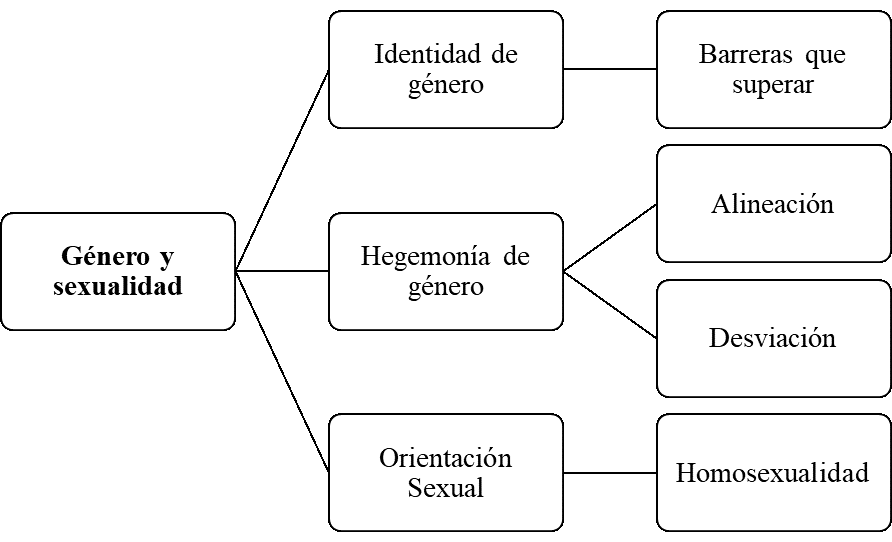
\includegraphics[width=0.75\textwidth]{genero}
    \caption{Diagrama de ‘género y sexualidad’}\label{fig:genero}
\end{figure}

\subsubsection{Identidad de género}

Esta subcategoría se mostró como la más importante dentro de lo expresado por
los participantes principalmente porque ha sido el componente central con
el que se enfrentaron en la constitución de su identidad. Esto se puede ver
reflejado en lo expresado por el caso~2:

\begin{verbatim}
…el momento más feliz de mi infancia es cuando me pude vestir
de Ángel Gabriel en un nacimiento viviente que hicieron en mi escuela. Mi mamá
no quería pero yo me sentía en las nubes porque por un momentito pude verme como
quería.
\end{verbatim}

Este conflicto de identidad también se hace visible dentro del relato del caso~3
cuando expresa:

\begin{verbatim}
…no es que solo me gustaba vestirme como hombre, es que pensaba
como uno también.
\end{verbatim}

Así como dentro del relato del caso~1 cuando comenta:

\begin{verbatim}
Cuando era pequeña no me molestaba, pero cuando empecé a
desarrollarme le rezaba a Dios para que por favor me salieran senos.
\end{verbatim}

Estos verbatims permiten identificar algunos aspectos relacionados con el
conflicto de identidad de los individuos. Elementos como el verbatim expresado
por el caso~2 que considera un recuerdo muy feliz el poder mostrar una
expresión de género acorde a la identidad que, ya para esa etapa de su
desarrollo, sentía era la de él. Además esto se puede reforzar con el verbatim
del caso~1 cuando expresa que le causaba preocupación y ansiedad el hecho que
sus senos no se desarrollaran junto con el resto de su cuerpo.

Además se presenta la dicotomía entre lo que las personas sienten que son, las
expectativas de como esperan verse y la imposición de la identidad que se
les asigno por haber nacido con un sexo especifico.

\subsubsection{Hegemonía de género}

Esta subcategoría surge de la relación que los participantes han tenido con
elementos propios de los roles de género, especialmente del rol del género
asignado según su sexo biológico. Es decir, está compuesta por aquellos
elementos que demarcan la diferencia entre lo femenino y lo masculino. Elementos
dentro del relato del caso~1 hacen presentes estas diferencias:

\begin{verbatim}
…el niño Jesús me dejaba una carta explicando que eso eran cosas de niña y me
traía patineta, bicicleta, carritos y a mí no me gustaba…
\end{verbatim}

Así como lo expresado por el caso~3:

\begin{verbatim}
Me decían que tenía que sentarme bien y como niña, y yo me preguntaba ¿cómo es
eso?
\end{verbatim}

Partiendo de estos verbatims se puede observar que existe un modelaje hacia el
individuo sobre el conjunto de expectativas especificas relacionadas con cada
género. Además se evidencia la insistencia de parte del entorno social por
conformarse a aquellas expresiones de género propios del género que les fue
asignado por su sexo biológico en el momento del nacimiento.

En estos verbatims se pueden observar, además, que existe una atribución, bien
sea masculina o femenina, sobre cosas (juguetes), o actos comportamentales.
Estas atribuciones son arbitrarias, pues en el caso del verbatim del caso~1,
los juguetes que le regalaban podían también ser asociados como juguetes de
niñas o en el caso del caso~3, que condiciones especificas son las que
determinan el como se debe sentar una persona dependiendo de su sexo o género.
Esto forma parte de los roles y expresiones de género, y son los primeros
elementos a los que los participantes parecen demostrar rechazo.

\subsubsection{Orientación sexual}

El último componente de la categoría de Género y sexualidad es la subcategoria
de ‘Orientación Sexual’. En esta subcategoría se presentan aquellas inquietudes
e incongruencias que surgieron en la vida de los individuos al momento de buscar
pareja sexual y romántica. No solo fundamentado en aspectos físicos sino también
emocionales. El caso~3 relata:

\begin{verbatim}
 Yo solía tener sexo telefónico con una amiga en bachillerato y en una de esas
 fantasías yo era un hombre y ella lo seguía y esas cosas sucedían y el primer
 nombre de mi personaje fue Alex y ahí empezó a asomarse algo que se transformó
 en lo que soy ahora.
\end{verbatim}

Este verbatim asoma un elemento resaltante de la orientación sexual en personas
transgénero, su consolidación se hace presente durante la adolescencia,
permitiendo de esta manera influir en la constitución identitaria del individuo.
Esto parece ser un elemento compartido en común tanto entre personas cisgénero
como transgéneros.

Así se puede interpretar que la personas trans dan muestras de su identidad de
género incluyéndole en los juegos sexuales de exploración tempranos. Reforzando
la idea de que estos presentan preferencia por presentarse según su género
sentido desde muy temprano en su vida.

Existe además una confusión asociada a la expresión de la sexualidad cuando no
se tienen interiorizados los conceptos propios de lo transexual o transgénero.
El caso~3 afirma al referirse sobre su experiencia sexual temprana:

\begin{verbatim}
Al principio todo hombre trans se cree lesbiana.
\end{verbatim}

El caso~2 refuerza esta confusión:

\begin{verbatim}
…yo no conocía de lo trans ni nada, pensaba que era homosexual y ya…
\end{verbatim}

Esto refuerza la concepción de que la orientación puede ser confundida con la
identidad, sobre todo cuando no existe un concepto claro de la transexualidad o
transgenerismo en la persona.

\subsection{Discriminación}

Esta categoría representa el segundo elemento más importante según lo expresado
por los participantes. La discriminación parece encontrarse inevitablemente
ligada a la condición trans. Los eventos discriminantes a los que ellos se ven
sujetos abarcan desde situaciones de rechazo como las que el caso~1 hace
presentes:

\begin{verbatim}
La población trans está muy expuesta al rechazo, porque no nos entienden,
piensan que somos unos bichos raros y nos ven y tratan como tales.
\end{verbatim}

Estas situaciones pueden llegar a convertirse en actos de acoso o bullying como
los que comenta haber vivido el caso~2:

\begin{verbatim}
Cuando inicié mi transición los compañeros de trabajo de mi papá se metían
conmigo, hasta que un día les ofrecí unos golpes y todo cambió.
\end{verbatim}

 Puede incluso llegar a generar en el individuo miedo así como una sensación de
 inseguridad como lo expresa el caso~3:

 \begin{verbatim}
Estando en Ecuador supe de un trans al que violaron y mataron y la verdad me dio
miedo.
 \end{verbatim}

Con base a estos verbatims se puede establecer un punto de referencia que
permite generar subcategorías en lo que se puede considerar una categoría
principal denominada \emph{Discriminación}. Los componentes de esta categoría se
pueden observar en la figura~\ref{fig:discriminacion}. Así mismo partiendo de
estos verbatims se puede pensar que las experiencias discriminantes son
trasversales a la vida de una persona transgénero ya que se pueden presenciar
tanto en etapas tempranas como en etapas mas adultas de la vida de los
participantes como se presenta a continuación.

\begin{figure}
    \centering
    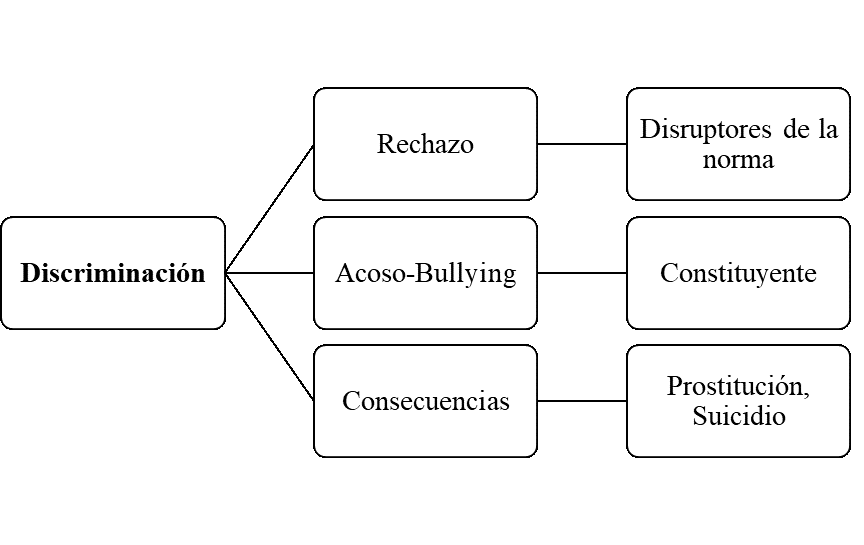
\includegraphics[width=0.75\textwidth]{discriminacion}
    \caption{Diagrama de categoría ‘discriminación’}\label{fig:discriminacion}
\end{figure}

\subsubsection{Rechazo}

Un elemento común en el discurso de los participantes es la presencia de
vivencias de rechazo, es decir situaciones en las que han sido víctimas de actos
que impiden su participación regular como miembro de la sociedad y que pueden
atentar contra la integridad de un individuo. Esto se hace evidente dentro del
relato del caso~2 cuando expresa:

\begin{verbatim}
Yo solía ir a comprar ropa de hombre y las vendedoras me decían que no. Porqué
compraba eso si yo era mujer y me miraban como con asco y yo les respondía que
lo hacía porque me gusta la ropa y porque tengo la plata para hacerlo.
\end{verbatim}

Así como también dentro del relato del caso~1 cuando comenta que:

\begin{verbatim}
…era horrible cuando me tocaba sacarme la cédula y me obligaban a ir vestida
como hombre, el personal que me atendía se ponía muy hostil conmigo cuando
llegaba maquillada.
\end{verbatim}

Estos verbatims permiten visibilizar elementos discriminantes que afectan la
expresión de identidad de género de los individuos transgénero. El rechazo que
pueden vivir parece tener sus raíces en condiciones socialmente construidas
relacionadas con lo que se espera que sea la expresión de género de una persona
de sexo masculino o femenino. Esta identidad que se le impone a las personas
transgéneros (sin importar su etapa de transición) afecta en contra del proceso
que transitan, generando malestar en el individuo. Debido a su decision de
alinear su expresión de género con la identidad de género con la cual se sienten
identificados se ven criticados y despreciados por comentarios como los
expresados por los participantes.

\subsubsection{Acoso / Bullying}

Otro elemento importante dentro de la vivencia de la discriminación por parte de
los participantes la relación que ellos desarrollan con el acoso o el bullying.
El caso~1 expresa que:

\begin{verbatim}
…en la escuela era algo terrible por el bullying, pero yo siempre imponía
carácter y jamás me deje amedrentar por nada ni nadie. De hecho me agarre a
golpes y me expulsaron por 10 días…
\end{verbatim}

Esto demuestra que desde etapas tempranas de su vida se encuentran presentes
elementos de acoso. El caso~2 expresa en su relato también que las situaciones
de acoso se pueden vivir en ambientes académicos:

\begin{verbatim}
Mientras estudiaba para sacar mi título de sexólogo me pasó que una docente era
particularmente agresiva conmigo, porque una vez le respondí feo. La razón de
esto fue porque ella estaba cuestionando mi identidad. Pero nada al final le
saqué un 20 y le callé la boca.
\end{verbatim}

Resalta el hecho de que, por su condición como personas transgénero, hechos como
el acoso o el bullying se hagan presentes con gran peso dentro del relato de los
participantes. Es también importante evaluar las estrategias con las cuales los
participantes lidian con estas situaciones. Parece ser que dependiendo del tipo
de acto que vaya en contra de ellos, ya sea violencia física o simbólica, para
poder ser redimido o valorado positivamente es necesario rebasar o exceder
aquellas expectativas que han sido impuestas por el agresor hacia el agredido.
Esto podría acarrear consecuencias negativas para la persona transgénero pues
vivir con la constante presión de tener que ser valorado solo por sus logros
puede llegar a ser una fuente de estrés negativo en la vida de la persona
transgénero.

\subsubsection{Consecuencias}

Por último es necesario remarcar que tanto el rechazo como el acoso o bullying
tienen consecuencias en las vidas de la persona trans. Por ejemplo, el caso~2
relata:

\begin{verbatim}
Hace poco supe de un caso de una chica trans, ella aún no comenzaba con su
tratamiento hormonal pero ya estaba expresando una identidad de género con la
que se sentía cómoda. La cosa es que por ser trans su familia la botó de la casa
y terminó en situación de calle, prostituyéndose para sobrevivir hasta que la
mataron hace una semana, la encontraron en un monte.
\end{verbatim}

Además se puede tomar en cuenta el comentario del caso~1, quien labora en una
oficina de atención social:

\begin{verbatim}
…aquí nos llegan muchos casos de personas trans que se quedan sin casa o trabajo
por querer ser felices, principalmente pasa con chicas, algunas se terminan
suicidando…
\end{verbatim}

 Esto pone sobre la mesa las consecuencias negativas que tienen situaciones
 aversivas producto de la discriminación. Estas siempre son una sombra de temor
 sobre la vida de las personas trans y es lo que les pone en riesgo de
 situaciones como la prostitución o el suicidio. Estas consecuencias tienen su
 origen en los elementos anteriormente mencionados en las subcategorías previas.
 Tanto vivir el rechazo por parte de otras personas así como el acoso y la
 necesidad de tener que encontrar estrategias de supervivencia que permitan al
 individuo valorarse ante otros como par hace que la vida de las personas
 transgénero este cargada de dificultades.

\subsection{La Transición}

En esta categoría agrupamos los elementos relacionados con el tránsito entre un
género o sexo a otro. Usualmente del género o sexo asignado al nacer hacia el
género o sexo deseado. Los elementos componentes de esta categoría se pueden
apreciar en la figura~\ref{fig:transicion}. Estos incluyen la elaboración que
realizan los participantes del proceso de transición en sí mismo desde su
subjetividad, la apariencia física y el conocimiento sobre los procedimientos
médicos, quirúrgicos y sociales que permiten llevar a cabo la transición.

\begin{figure}
    \centering
    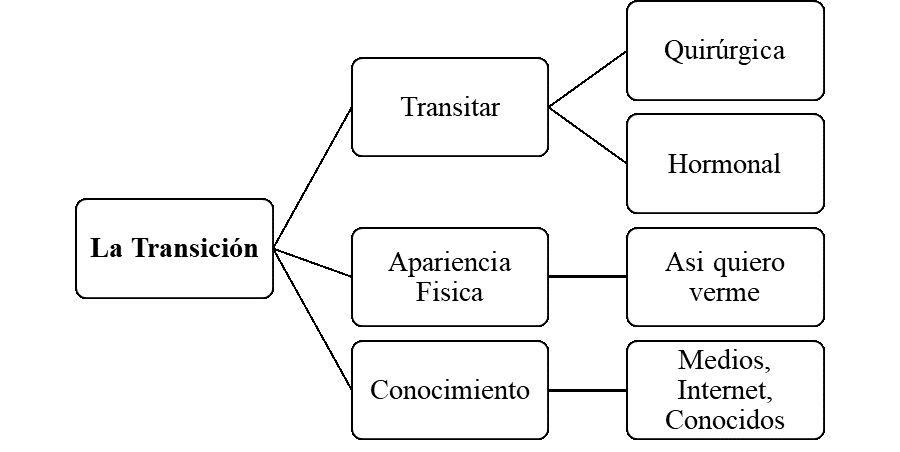
\includegraphics[width=0.75\textwidth]{transicion}
    \caption{Diagrama de ‘la transición’}\label{fig:transicion}
\end{figure}

\subsubsection{Transitar}

Según lo expresado por los participantes, el transitar va mas allá de se un
simple hecho sino que también es una herramienta. La transición es un medio que
les permite llega a ser quien ellos sienten que realmente son. El transitar
puede abarcar aspectos quirúrgicos y/u hormonales, y como lo expresa el caso~2:

\begin{verbatim}
…las hormonas ayudan pero la operación libera…
\end{verbatim}

El caso~3 coincide al comentar:

\begin{verbatim}
…las hormonas ayudan, cuando dejé de tomarlas perdí todo, era una niña…
\end{verbatim}

Estos comentarios evidencian que existe una valoración de la alteración
quirúrgica como más importante que el tratamiento hormonal. Además se considera
la transición quirúrgica como un objetivo final o como una acción liberadora.

Sin embargo, lo dicho por el caso~3 hace referencia a como el componente
hormonal tiene una importancia por su cualidad inmediata. Debido a que permite
una visibilización a corto plazo de la identidad, mas explícita que una
operación. Los efectos de la transición hormonal son visibles mientras que la
cirugía genital no lo es. De igual manera, el tratamiento de reemplazo hormonal
requiere de una toma constante. Por ello dejar de tomarlo implica una reversión
rápida de sus efectos.

Por otro lado se tiene que tomar en cuenta lo expresado por el caso~1:

\begin{verbatim}
…por cuanto mi apariencia física y genética me han ayudado en la transición lo
cual ha sido muy fácil, de hecho no he tomado hormona nunca…
\end{verbatim}

Esto permite indicar que la importancia no está colocada en la toma de hormonas
en sí mismo. Sino que la importancia está en los cambios de aspecto físico y de
visibilidad que se producen como resultado de la influencia hormonal. En esta
instancia el caso~1 indica no necesitar de la toma hormonal pues su aspecto ya
es femenino en sí, lo que es su objetivo último.

Este elemento se relaciona con la Apariencia física, pues es el aspecto—
efectivamente la expresión de género— lo que la persona trans desea alterar. La
función biológica es secundaria a sus efectos sobre la expresión.

\subsubsection{Apariencia física}

Aquí podemos encontrar la expresión de la relación sexo-género. Es decir, la
relación existente entre el género y las caracterísitcas sexuales secundarias.
Se debe tomar en cuenta que dentro de esta relación hay particularidades que
tienen un mayor peso o que suelen tomarse más en cuenta para su expresión como
lo plantea, por ejemplo, el caso~3 al referirse a un tiempo en el cual dejo de
tomar hormonas:

\begin{verbatim}
  …perdí el torso perdí básicamente eso, la libido cambio…
\end{verbatim}

Esto implica que el poder verse y expresarse en concordancia con los rasgos del
sexo o género al que se transita es fundamental. Además de que también tiene
importancia el cómo se siente. Aquí refleja uno de los efectos de la
testosterona sobre el impulso o deseo sexual. No sólo desea verse, sino sentir
su propio cuerpo como aquel del sexo deseado.

Además de esto se puede tomar en cuenta lo expresado por el caso~2:

\begin{verbatim}
…le tengo terror a la regla porque soy hombre y a los hombres no les debe venir
eso.
\end{verbatim}

Este refleja la importancia del ‘sentirse como’. No se trata, sin embargo, de
una búsqueda funcional. La menstruación como fenómeno biológico tiene un
objetivo reproductivo. No es la función o la menstruación lo que rechaza el
participante sino el desarreglo con la conformación estereotípica de la
dicotomía sexual. No se rechaza el tener la menstruación sino el hecho de tener
la menstruación siendo hombre. Esto no se ajusta con la construcción física
propia del hombre y por ello es rechazado.

Este elemento visibiliza la concepción de concordancia de sexo/género que
prevalece, pues estar alineado no solo puede significar tener características
propias de un sexo o género, sino que también puede significar no tener o evitar
las asociadas con otro.

\subsubsection{Conocimiento}

La subcategoría de conocimiento hace referencia tanto a cómo los participantes
reafirmaron o conocieron su condición así como a la manera con la cual entraron
en contacto con el proceso que les permitiese su transición. En esta
subcategoría resalta el papel de los medios para visibilizar la
condición trans, el caso~2 expresa que:

\begin{verbatim}
…yo no conocía de lo trans ni nada, pensaba que era homosexual y ya, pero
luego un día viendo televisión con mi novia de ese momento pasaron el primer
capítulo del programa ‘Taboo’, por NatGeo y ahí presentaron a una persona trans
y mi novia me dijo, mira ella dice que se sentía como tú dices que te sientes
y pues eso me dejó pensando.
\end{verbatim}

Podemos entonces afirmar que hay aún un desconocimiento de la diferencia entre
la orientación sexual y la identidad sexual. Además, se evidencia que es
necesario para la personas trans aprender e interiorizar los significados de:
género, sexo, identidad sexual y transición, para poder dar sentido a la propia
experiencia. Sin estos significados no es posible para la persona trans comenzar
a poner en cuestionamiento el género asignado y la propia identidad.

Por otro lado se puede tomar como referente la experiencia del caso~1 que
expresa:

\begin{verbatim}
Me di cuenta y logré comprender que era ser trans a los 40 años de edad, porque
desconocía que era ser trans, de hecho en mi ignorancia tampoco sentía que me
identificaba como gay porque me sentía mujer pensaba como mujer y eso no lo
entendía, todo eso lo viví en silencio por 40 años jamás dije nada por el
rechazo que pudiera sentir hasta que me hablaron de personas trans y fue allí
cuando comencé a entender que yo era una mujer transexual.
\end{verbatim}

Esto refuerza la diferencia entre la orientación y la identidad sexual. También
señala la vivencia privada y subjetiva de la mayoría de las personas trans
quienes suelen mantener su confusión en silencio por miedo al rechazo. Refuerza
también la importancia de la comunicación de los conceptos alrededor del género
y la identidad para poder asumirse a sí mismo como persona trans.

El caso~1 añade:

\begin{verbatim}
Lo descubrí a los 40 años gracias a mi psicólogo que me realizo una terapia y
allí fui abriéndome y diciendo lo que sentía y fue cuando supe que era una mujer
trans.
\end{verbatim}

Esto potencia el rol del psicólogo como voz autorizada y mediador en el proceso
de transición, calmando el malestar del individuo. El psicólogo aquí también
ejerce la función de educador de la persona con un malestar que no ha podido
significar o expresar de una manera satisfactoria. La adquisición de conceptos
psicológicos y los símbolos propios de la identidad de género le permite a la
persona trans construir su propia interpretación de su condición e identidad.

\subsection{Cuerpo y genitalidad}

Esta categoría se centra en el aspecto biológico de la identidad del individuo
pero no abarca componentes hormonales o cromosómicos como tales sino que se
centra únicamente en el aspecto fenotípico genital desde lo estético y lo
sensitivo así como lo que representa para los participantes este aspecto de su
cuerpo.

En la figura~\ref{fig:genitalidad} se pueden observar los componentes de esta
categoría.

\begin{figure}
    \centering
    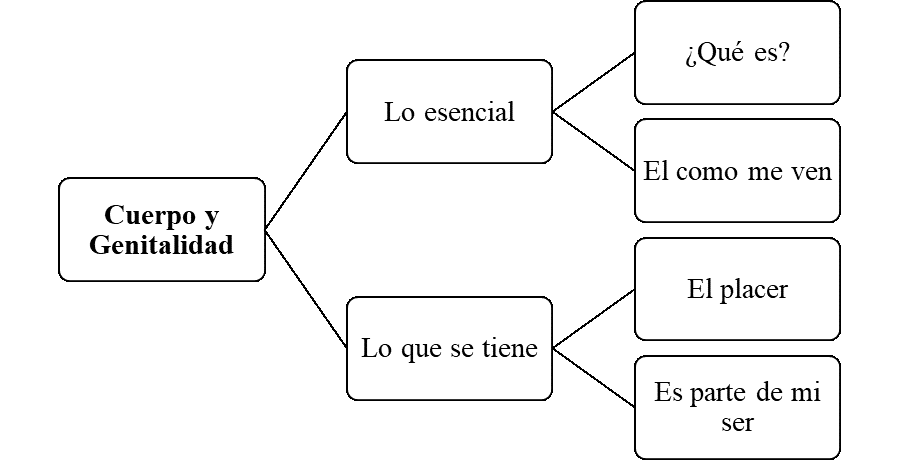
\includegraphics[width=0.75\textwidth]{genitalidad}
    \caption{Diagrama de ‘genitalidad’}\label{fig:genitalidad}
\end{figure}

\subsubsection{Lo esencial}

Esta subcategorías abarca aquello que los participantes consideraron de mayor
importancia sobre su relación con el cuerpo, es interesante observar que el
componente genital no tiene una primacía en la construcción de su identidad. Si
se toma en cuenta lo expresado por el caso~1 cuando se le pregunta por la
transición quirúrgica:

\begin{verbatim}
Solo me decidí operar el pecho y ponerme mamas.
\end{verbatim}

Esto es resaltante porque aunque el sentirse como perteneciente al género
deseado es importante, aún más importante es ser recibido y aceptado socialmente
como el género con el cual se identifica. En este sentido la opción quirúrgica
es evaluada en su función para la expresión del género deseado, y por ello se le
da prioridad a la mamoplastia.

También el caso~3 comenta:

\begin{verbatim}
¿Para qué un trans se opera el pecho? para poder quitarse la camisa.
\end{verbatim}

Y el caso~2 agrega:

\begin{verbatim}
Quiero poder operarme para poder quitarme la camisa y hacer cosas normales.
\end{verbatim}

Una vez más se ve reforzado que el cambio corporal esencial es aquel que permite
la inserción social. Parece resaltar la importancia de lo que se considera
caracteres sexuales secundarios sobre los primarios. Es decir, es más importante
lo que ve el otro en público que lo que se ve en privado. Comentarios como el
del caso~2:

\begin{verbatim}
…a mí me encanta ir al gimnasio y tener la espalda ancha, me
siento como un monstruo.
\end{verbatim}

Refuerzan la idea de que lo esencial es mostrarse para todos y ser recibido cómo
el género con el cuál hay identificación. Aquí el uso de monstruo es un sentido
positivo. Desde la mirada que asocia a un ‘monstruo’ con fuerza, tamaño físico,
poder y vitalidad. Características estereotípicamente asociadas con la
masculinidad. Además de que la idea que yace detrás es la realización de las
interacciones sociales típicas del rol de género por el que se desea pasar. En
este caso, el hombre que va al gimnasio es para hacerse fuerte, muscular, grande
y poderoso.

\subsubsection{Lo que se tiene}

Además de lo encontrado en la subcategoría anterior los participantes expresaron
que es más importante el genital que se tiene, y como este permite relacionarse
con una pareja, que buscar que los genitales coincidan con el género con el que
se identifican. Es por esto que la presente subcategoría nace, tomando en cuenta
comentarios realizados por los participantes, como por ejemplo lo expresado por
el caso~3:

\begin{verbatim}
Lo mío es mío y con esto resuelvo.
\end{verbatim}

A lo que le agrega:

 \begin{verbatim}
…un pene falso a nivel sexual es solo un instrumento.
 \end{verbatim}

También comenta el caso~2 sobre la cirugía de reasignación de sexo:

\begin{verbatim}
Eso después hace que pierdas sensibilidad
\end{verbatim}

Se puede interpretar de estas expresiones que existe una preferencia a acercarse
a la relación sexual desde los genitales con los que se nació. La genitalidad
propia del género con el cuál se sienten identificados es un aspecto secundario.
A esto se le puede sumar la importancia asignada a la cirugía de mamas, ya sea
para removerlas o crearlas. Esto está relacionado al valor exclusivamente
femenino que tienen los senos en la sociedad como un aspecto visual y evidente
que señaliza la femineidad.

\subsection{El Otro}

Esta categoría fue nombrada debido al peso que tiene la presencia del otro en
la vida de cada individuo dentro de la sociedad. Debido a que el ser humano es
un ser intrínsecamente social existen principios que rigen las interacciones así
como diversas formas para poder satisfacer las necesidades que surgen de estas
interacciones. Tomando en cuenta que la condición trans puede ser disruptiva
dentro de lo socialmente aceptado se puede comprender que la importancia del
otro cobra un sentido particularmente fuerte en estos casos pues el otro puede
moldear la forma en la que se asume el género así como patrones de
comportamientos, vestimenta y roles que permitan al individuo expresarse según
el género con el que se sienten identificado.

En la figura~\ref{fig:otro} se puede observar la estructura de los elementos que
componen esta categoría.

\begin{figure}
    \centering
    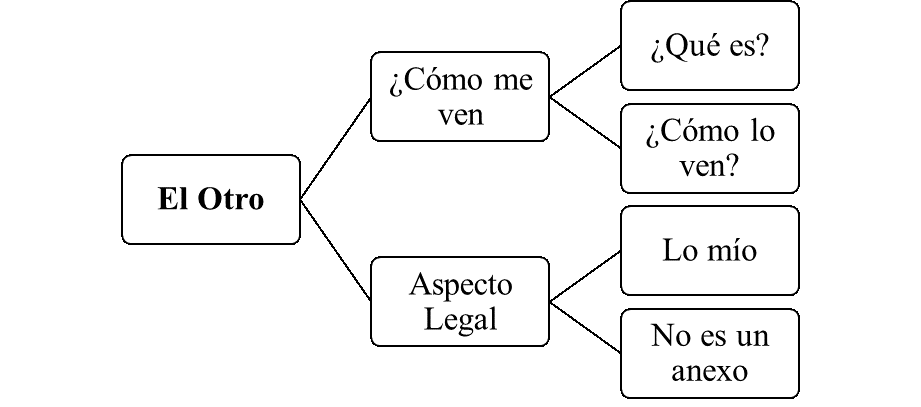
\includegraphics[width=0.75\textwidth]{otro}
    \caption{Diagrama de categoría ‘el otro’}\label{fig:otro}
\end{figure}

\subsubsection{Cómo me ven}

La primera subcategoría es sobre la percepción general que tienen los demás de
la persona transexual, o al menos cómo estos la conciben. Tomando en cuenta lo
expresado por el caso~3:

\begin{verbatim}
  …me solían ver como el raro…
\end{verbatim}

Caso~1:

\begin{verbatim}
Les causa impresión y cambia todo cuando doy mi cedula para pagar maquillaje.
\end{verbatim}

Parece ser que el rol transgresor de la condición trans es lo que permea el
trato que estas personas reciben. Es decir, cuando alguien interactúa con una
persona trans el saber o no que se encuentra hablando con una persona trans va a
afectar el trato que reciban. Además, el trato que reciben es percibido como
regular hasta que la otra persona se da cuenta que está interactuando con
alguien trans,

El caso~2 agrega:

\begin{verbatim}
La gente juzga mucho y como que esperan más de ti, que seas más hombre que otro
hombre o más mujer que otra mujer.
\end{verbatim}

Esto apunta como la persona trans se ajusta a la mirada de los otros por medio
de asumir expresiones propias del género con el que se encuentran identificados.
Bien sea mediante comportamientos o alterando su apariencia física. Resalta el
calificativo utilizado por el caso~2 ‘más hombre que otro hombre o más mujer
que otra mujer’. Esto implica que existe una presión y una expectativa por
cumplir con los estereotipos de los roles de género. Incluso más allá de lo que
sería razonable para una persona cisgénero.

Cabe señalar en este aspecto un comentario realizado por el caso~3:

\begin{verbatim}
Yo llevo un aparatico para poder usar el baño de hombres, porque sabes los
hombres se miran a veces y a mí me gusta usar un urinario y orinar de pie.
\end{verbatim}

Este relato entra en contacto con lo expresado por el caso~1:

\begin{verbatim}
Yo soy muy coqueta, me hice así una vez me asumí mujer trans, antes no me
arreglaba mucho.
\end{verbatim}

Parece ser que el adaptar o incluir roles de conducta propios de un género no es
un hecho exclusivo para la aceptación privada, sino es también un elemento
de validación con el otro.

\subsubsection{Aspecto legal}

Complementando a la subcategoría anterior se presenta el ‘Aspecto legal’, que
indica la forma en la cual son reconocidos legalmente las personas trans. Este
es un elemento constitutivo de su identidad debido a que al ser ciudadanos de la
Republica Bolivariana de Venezuela necesitan contar con la seguridad legal de
que sus derechos van a ser respetados y el primer paso es poseer una identidad
legal, como el caso~1 lo expresa:

\begin{verbatim}
…otro momento en el que fui muy feliz fue cuando pude sacarme la foto de la
cédula con maquillaje y expresándome como soy de verdad.
\end{verbatim}

El poder ser identificada legalmente según su expresión de género es algo muy
significativo pues los reafirma como ciudadanos con derechos. Si bien el cambio
de sexo en la identidad no es posible aún, ser reconocido en la fotografía de su
identidad y aparecer cómo realmente se expresan en el día a día representa una
pequeña victoria. El caso~2 refuerza este planteamiento comentando que:

\begin{verbatim} …cuando legalmente se nos pueda identificar sin ningún problema
pero va a ser una victoria muy importante, el siguiente paso sería quitarnos el
prefijo trans, yo soy un hombre y ya no un hombre trans, eso no es inclusivo.
\end{verbatim} % FIXME sin ningún qué?

\section{Discusión}\label{sec:discusion}
% NOTE Emerson hará intro y primeras tres categorías

Cuando se inicio la presente investigación se plantearon unos objetivos que
buscaban enfocar los significados asociados la transición por personas Trans
desde una mirada no patologicista, por esto se estructuró todo el proceso de
recolección de datos e interpretación de los mismos desde una metodología
cualitativa. Principalmente la necesidad de romper con la noción de la condición
trans como una enfermedad mental (forma como ha sido catalogada desde
aproximadamente la década de los ochenta según manuales de diagnostico como el
DSM-IV y el CIE-10) fue el catalizador para que surgiera la presente
investigación. Además de esto se presenta al rol del psicólogo como voz
autorizada permitiendo la comprensión o legitimización de las prácticas de cada
persona o grupo de individuos en este caso.

Podría asumirse que gran parte de las dificultades para la integración de las
personas trans nacen de la forma en la que se han construido las identidades en
la sociedad, por medio de dicotomías rígidas que facilitan la patologización de
expresiones humanas que se salgan de lo “establecido”. Esto entra en contraste
con respecto a lo planteado por proposiciones como la Teoría Queer, que como lo
explican Fonseca y Quintero (2009) asume a la expresión de género como un
continuo, si bien pueden existir extremos no son más que puntos de referencia,
marcadores, entre los cuales se pueden encontrar las diversas expresiones de
género y sexualidad de el ser humano. Al tomar esto en cuenta parece ser posible
complejizar la condición trans y verla como un hecho que al ser apologizado
puede estar reduciendo la verdadera complejidad del asunto.

El reduccionismo del que es víctima la condición trans podría verse sustentado
en Venezuela por el limitado número de investigaciones sobre este tema que
existe en la actualidad y que busca romper con la idea de la condición trans
como una condición patológica. El hecho que existan pocas investigaciones
también puede ser síntoma de que en Venezuela no se visibiliza con facilidad el
proceso que conlleva la condición trans, es decir, aquellas personas que deseen
transitar de un género o sexo a otro a veces no cuentan con la información
necesaria o el apoyo para lograr este proceso. Esto hace que se invisibilice a
la población trans, al existir poca comprensión sobre la condición se le suele
confundir con homosexualidad o incluso se puede llegar a llamar a una persona
trans “travesti”, caracterizando a las personas trans como “anormales”, de nuevo
todo esto enmarcado en una dicotomía de la identidad.

Identidad que para los participantes se construye de una manera específica,
marcada por las interacciones que se llevan a cabo en su cotidianidad, desde su
infancia hasta su adultez.  Estas vivencias en su infancia se convierten en los
cimientos que moderarán la forma en la que se desenvolverán en la sociedad, es
necesario remarcar que la condición trans en estos individuos es asumida no como
una elección, sino como algo que es, no es un capricho o moda, es un sentir real
y autentico que en muchos casos los lleva a un estado de conflicto pues no se
logra encontrar como balancear la identidad sentida y lo socialmente esperado.

Precisamente el romper con lo socialmente aceptado causa que sean vistos como
“anormales” o con una identidad falsa y los lleva a asumir posiciones de defensa
de su integridad como individuo, defendiéndose de comentarios emitidos por
miembros de sus familias, compañeros de clases e instituciones, estos actores no
solo pueden constituir en algunas ocasiones el principal obstáculo con el que
tienen que lidiar las personas trans, sino que también actúan como perjuradores
dentro de las actitudes y prejuicios dirigidos a la población trans.

El rol de estos actores pone sobre la mesa la importancia del otro en la
constitución de la identidad de un individuo, pues es el otro aquel que
recrimina y exige un comportamiento específico (principalmente ligado al género
asociado con su sexo de nacimiento). El otro actúa también como determinante
para poder entrar en contacto con la condición trans, el ser diferente a lo
considerado “normal” permite en la persona trans una identificación según
aquello que “les falta” o “les sobra”. Desde una mirada teórica se puede tomar
como referencia lo planteado Hernández, Rodríguez y García-Valdecasas (2010)
para explicar desde una perspectiva clínica la razón por la que el otro puede
sentir un rechazo muy marcado ante personas trans y es porque se suele asumir
que alguien que no se adapte o asuma los modelos y roles determinados
socioculturalmente según el género asignado por el sexo biológico es un
individuo anormal. Paradójicamente esta visión deja de lado los elementos
sociales que plantean que el género no es un elemento rígido e inmutable sino
que es socialmente construido, al tomar este elemento en cuenta se puede ampliar
la dicotomía macho/hembra.

Este interés en poder ser aceptado hace que lo publico pese más que lo privado
al momento de constituir la identidad de una persona trans. Según lo encontrado
en las entrevistas lo primordial para sentirse cómodos como individuos es tener
una expresión adecuada, comentarios como el de caso~2 y caso~3 hace presente
esto, expresando su interés en poder ser vistos en contexto sociales realizando
acciones asociadas con la masculinidad, en el caso de caso~2 poder quitarse la
camisa en la playa o no utilizar sostén, y caso~3 expresando que desea
mantener una figura masculina. Caso~1 también expresa esto haciendo referencia
a la importancia que tuvo para ella realizarse una cirugía de aumento de mamas
decidiendo no hacer tratamientos hormonales o llevar a cabo otras cirugías.

El caso de caso~1 trae a luz un elemento importante y es que la condición
trans no necesariamente tiene que verse ligada con reasignación de sexo por
medio de cirugías o el tomar algún tratamiento hormonal. Parece ser más
importante la visibilización de uno ante los otros que otros elementos, quizás
el tratamiento hormonal y las cirugías permitan un mayor acercamiento a la
auto-identificación pero no son necesariamente obligatorios. Es más una
condición de aprender a ser hombre o mujer que a tener elementos propios de
ellos.

Esto se hace visible en la relación que los participantes han desarrollado con
su genitalidad. Caso~3 hace referencia a que prefiere mantener los genitales
que posee a tener que realizarse una faloplastia, tomando en cuenta que primero
podría ser poco atractivo estéticamente y que podría además significar una
pérdida de sensación, sin embargo hace referencia también a que valora mucho el
poder orinar de pie usando un embudo que guarda entre sus piernas y que
visualmente (desde el otro) se puede asumir como un pene.

Este aspecto (es poder ser considerado hombre o mujer) entra en contacto con una
realidad presente en la sociedad y es la primacía del hombre sobre la mujer
desde el patriarcado. Autores como Lenner (1990) expresan que el patriarcado es
un sistema en el que los roles de género se encuentran claramente marcados y
segmentados. Es por esto que el relato de caso~1 contrasta contra los de
caso~2 y caso~3 pues para ella el asumirse mujer fue un proceso más arduo
que para ellos asumirse hombres, principalmente porque adaptarse a los roles de
género es más complicado debido a las exigencias impuestas a las mujeres
socialmente, es decir el tener que verse femenina puede ser un reto cuando
durante casi toda su vida el tener que arreglarse no tuvo un peso realmente
determinante en su vida. Por otro lado caso~2 y caso~3 expresan que tener
que asumir roles masculinos va ligado con la presencia de musculatura, un cuerpo
visualmente masculino les permite desarrollarse con normalidad en la sociedad.

Parece importante resaltar que la identificación que hacen los participantes con
los géneros va ligados a estereotipos y que tomando en cuenta lo planteado por
la teoría queer se podrían expresar en un continuo, sin tener que empeñarse en
asumir un extremo o el otro de manera rígida.

En definitiva, se podría afirmar que los individuos independientemente de sus
experiencias parecen construir una identidad más enfocada en lo que el otro
puede ver y juzgar que no necesariamente abarca aspectos más privados como los
genitales,  por esta razón ellos (las personas trans) transcienden las barreras
de sexo y género con la contradicción de que en su identificación se les empuja
a asumir extremos rígidos para poder ser validados socialmente y poder evitar
prejuicios y discriminación.

% NOTE no exceder las 1000 palabras por categoría
\subsection{Desarrollo}
%
% \subsubsection{Infancia y pubertad}
%
% \subsubsection{Familia}
%
\subsection{Género y sexualidad}
%
% \subsubsection{Hegemonía de género}
%
% \subsubsection{Orientación sexual}
%
\subsection{Discriminación}
%
% \subsubsection{Rechazo}
%
% \subsubsection{Acoso / Bullying}
%
% \subsubsection{Consecuencias}
%
\subsection{La transición}

El concepto de la transición para los participantes

% \subsubsection{Transitar}
%
% \subsubsection{Apariencia física}
%
% \subsubsection{Conocimiento}
%
\subsection{Genitalidad}
%
% \subsubsection{Lo esencial}
%
% \subsubsection{Lo que se tiene}
%
\subsection{El Otro}
%
% \subsubsection{Cómo me ven}
%
% \subsubsection{Aspecto legal}
